% Analyse where the network misclassified (some examples) 
%remember we classify authors not tweets -> example would be author level
% Features that contribute the most (#hashtag) is usually used a denotation of irony. Vocab size (smaller for I), usually simple language. 
% Limitations: Context, while we attempted a simple embedding usage, our model currently has no context information.
% - While we avoided deep methods to allow for more interpretable features, the fact that half our points are resulting from PCA  means that it's not clear what some features are. 
% Our model might need some modifications to scale (namely the TF-IDF) as more data would require much more space to store the vectors. Clipping vocab could be used, stemming.
% Refer that due to the lack of tweet level labels it~s hard
% Considering different models learned through different features we could consider using an ensamble (merging probabilities of different models for different features).
% Author VS Tweet level and sample size. (How data is anotaded)
\subsection{Model Performance}

Our results show that the classifiers SVM, logistic regression and especially random forest perform very well with our features. Of the NN-classifiers, 3-NN performs best, but still lags a couple of percentage points behind the better-performing models. Our highest F1-score with random forest is 96.04, an F1-score that according to \citeA{sarcasm_detection}'s survey of the field is only topped by \citeA{ghosh2015sarcastic}, who obtain a score of 97.5 with a distributional semantics approach. 

Such high results are rather surprising considering the relative simplicity of the features used in our model. Especially the lack of semantic similarity or incongruity features (although perhaps sentiment SD could be interpreted as such), which are otherwise widely used \cite{reyes2012humor, riloff2013sarcasm, joshi2015harnessing, joshi2016word}, makes this a remarkable result.

However, considering that a simple char-gram model paired with SVM is able to obtain an F1 of 84.36, we suspect that this dataset is simply easier to classify than previous datasets in similar tasks. This might have to do with how this dataset was annotated and how the Twitter users were sampled. Unfortunately the task authors do not provide us with this information, so it's unclear what makes this dataset unusual. However, we do know that some ways of collecting twitter data, for example based on \#irony hashtags, can create datasets that are easier to classify \cite{sarcasm_detection}, so data collection and sampling methods likely play role here as well.

Unlike most previous research that focuses on the tweet-level irony detection \cite{sarcasm_detection}, we are classifying irony on the user level. This is significant, as previous research \cite{cyberbullying} shows that the majority of hate speech is produced by a small minority of people. It might therefore be more effective to identify hateful/sarcastic users than individual utterances. It might also be the case that identifying irony on the user level (both in terms of annotation and prediction) is more robust than doing so for individual tweets, and that this is partly responsible for the high F1-score. 

As seen in Table \ref{tab:test_results} the high scores were robust (and even improved) when only 70\% of the data was used for training. 

\begin{figure}[!h]
    \centering
    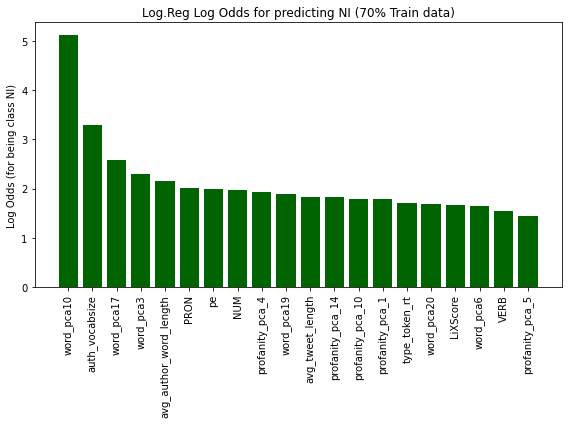
\includegraphics[width=0.48\textwidth]{images/NI_features_log_reg_odds.png}
    \caption{Log odds for predicting NI}
    \label{fig:ni_log_odds}
\end{figure}

\begin{figure}[!h]
    \centering
    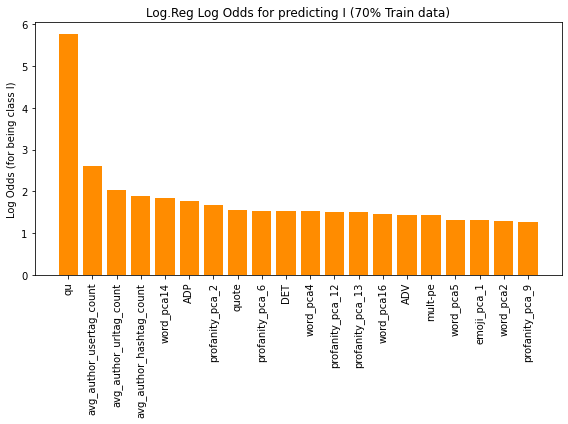
\includegraphics[width=0.48\textwidth]{images/I_features_log_reg_odds.png}
    \caption{Log odds for predicting I}
    \label{fig:i_log_odds}
\end{figure}

\subsection{Feature Peformance}

While developing our different features we found that even the stylistic count features on their own performed similar (about 80\% accuracy) to the Baseline model, despite being quite primitive. This means that simply by looking at the general stylistic characteristics of an author a machine learning model is able to separate the two classes. This indicates that the difference between ironic and non-ironic tweeting styles really is very distinct on the user level. Every other feature yielded small improvements, with TF-IDF being the highest contributor. 



Based on feature permutation (see Appendix), we found that vocabulary size, hashtag counts and question marks were among the most significant features, as well as some TF-IDF PCA vectors, i.e. stylistic and lexical features. This is consistent with previous studies \cite{gonzalez2011identifying, joshi2015harnessing} where lexical features (especially unigrams) are used a baseline and core of more complex models. Studies that find strong effects of punctuation and similar stylistic features include \citeA{bouazizi2015sarcasm} and \citeA{van2018exploring}. Per Table \ref{tab:cross_validation_results}, using the sentiment standard deviation rather than the mean also generally improved results by a small amount. The standard deviation might be better than the mean at capturing incongruencies in polarity, which are often indicative of irony. 

For a more fine-grained analysis, we find the log odds for predicting ironic and non-ironic users in Figure 3 and 4, respectively. We see that ironic users are characterized by a higher use of question marks, more URLs, usertags (replies) and hashtags, while non-ironic users have a larger vocabulary size and word length, among others. Some PCA features also increase the odds of being non-ironic, which again might be related to the larger vocabulary of those users.

While looking into the values of different words in the TF-IDF, we noticed that sometimes words specific to a single user, as for instance a promotion code, will have very high values in the TF-IDF vector, as they fit the criteria of being used by only a single user multiple times. For instance, in \verb'word_pca_10' when trained on 70\% of the data, if we softmax the weights on that PCA component and sort them according to their scores we find the following words score highest: `women', `:', `and', `men', `calm',  `gay', `guard', `code', `USER-PROMO-CODE'. As we can see, some words here might be related with irony and stereotypes, like `gay' and `women', but the user promotional code is not related at all to the task and might add noise. To ensure a better quality of these features, we could have opted for stemming and removing stop words or words that only appear in a single user (to capture cases like promotional posts), while accepting that we might lose some information.

%An observation furthered by the good performance of the baseline which is only based on char grams. It is interesting to see how these few relatively simple features can already lead to results as good.
% While we aimed to use classical machine learning methods paired with easy to understand features to discern patterns between the two classes, we still were in need of using PCA to reduce the dimensions of the large resulting TF-IDF vectors from this dataset. This means that a lot of the information provided by the PCA is not easy to interpret. We expect the resulting vectors to contain features that are used a lot in a few tweets and that vary a lot between different authors. 

% We used classical ML for explainable results. A analysis of each feature could give us an approximation about what an ironic style is. However, the majority of our features are based on PCA which reduces the explainability again as it is not necessarily clear what these features mean.

%author level 
Due to the nature of the task as an author classification task we cannot say if a particular tweet is ironic. Instead we are only able to classify by all their tweets, but not exactly point out where irony or stereotypes are present. However given the annotations for the dataset, one would have to identify specific cases of irony/stereotypes manually to allow for this type of classification. It is also not clear how many ironic tweets make a user an irony-spreader or not. Therefor is unclear how the system would perform in the wild or for larger datasets, when the annotation is not as clear or generated in other ways. 
 
\subsection{Limitations}

Our model has several limitations and areas for improvement. A general drawback is the time it takes to generate the features for the training and test data, particularly for the TF-IDF and profanity PCA features. This means the model would not scale well in terms of time and space usage. To avoid this scalability problem the number of terms for TF-IDF could be reduced by clipping the vocabulary or stemming the words in each tweet and accepting some information loss in exchange for a faster performing system.

Currently our model does not consider context. Our features at most capture a unigram language model by the usage of TF-IDF, but even then it's distorted by PCA. While we attempted embeddings, these were not beneficial to the task. This is a bit surprising considering the success others have had with word embedding-based features in conventional ML \cite{joshi2016word}. Word embeddings in isolation might not capture enough information, and would need to be processed in some way before being used in the model. They would also likely be more useful in a deep-learning approach, which is the type of model in which they are usually used \cite{zhang2019irony, sarcasm_detection}.

That being said, we believe our model would require features that encode semantic and pragmatic information, incongruencies or even ontologies to interpret if some words are being used out of the expected context

Another direction for future work relates to the fact that the different classifiers appear to rely on different features (see Appendix). Considering this, an ensemble method could be used to combine different classifiers to optimally use more of the features. We could for instance have a model that focuses on more low-level features, which word combinations are more likely, and a model like ours which uses more high-level and general features. 

% Mistakes:
% Probabilities are: I / NI
% c75bc1b6dd7d283e1ff17a2a8a512a76.xml : 0.09 / 0.91 (Correct label I) ⛔
% a7e7cc1908ee78179a883a47ae68c52f.xml : 0.5 / 0.5 (Correct label NI), Essentially this one was random ⛔
% e19408d8b77473ec2c23d11bd589e2fe.xml : 0.01 / 0.99 (Correct label I) ⛔The worst mistake
% ce6df51b12f065042c81f98ed0773687.xml : 0.49 / 0.51 (Correct label I) ⛔
% ceec7ed40f2ddeebd501ba2b785ff305.xml : 0.47 / 0.53 (Correct label I) ⛔
% 8ee99a8ea76169ee47b978f6cce69fb0.xml : 0.48 / 0.52 (Correct label I) ⛔
% 446a550e12709539e1af83c2dba75de7.xml : 0.01 / 0.99 (Correct label NI)✅
% 53405c12b5e86d2f3847850939d712b0.xml : 0.04 / 0.96 Correct Label (NI)✅
% 14c6666bf57dc5b6f5334ed8a65bffd4.xml : 0.97 / 0.03 Correct Label (I)✅

% Interesting find: "We don't buy bitcoin We earn bitcoin From Mining I'm ready to show 10 lucky people how to earn 0.1BTC" is repeated accross 5 users - what is this?

